
\section{Ergebnisse und Diskussion}\label{chap:results}

In diesem Kapitel werden die Ergebnisse der einzelnen Zwischenschritte der Methodik nach \autoref{chap:Methodik} dargestellt und kritisch betrachtet.
Hierzu gehören vorerst die Ergebnisse der Clusterung der \gls{MS}-Netzgebiete, die mit \gls{SIMBEV} erzeugten Fahrtprofile und Standzeiten von \gls{EPKW} und deren räumlicher Verteilung, sowie die Ergebnisse der Implementierung der verschiedenen Ladestrategien.
Abschließend erfolgt eine detaillierte Betrachtung der Ergebnisse der Ermittlung des Abregelungsbedarfes aufgrund der Integration von \glspl{EPKW} für die untersuchten Netze.


\subsection{Erzeugung und Charakteristik der Fahrtprofile}

Mit Hilfe des Software Tools \gls{SIMBEV} werden für die Referenznetzgebiet die Fahrtprofile der im Netzgebiet befindlichen Fahrzeuge erstellt.
Die Charakteristik der Fahrtprofile spielt eine entscheidende Rolle für die Wirksamkeit der unterschiedlichen Ladestrategien und die Auswirkungen auf die Netze.
Hierbei steht vor allem die Jahresfahrleistung der \glspl{EPKW}, der Anteil flexibilisierbarer und nicht-flexibilisierer Ladevorgänge, die Gleichzeitigkeit der Ladevorgänge und wann diese auftreten im Vordergrund.
Innerhalb dieses Kapitels werden die Ergebnisse der Regionalisierung dargestellt, sowie die Charakteristik der erzeugten Fahrtprofile kritisch betrachtet.
Dabei liegt der Fokus auf der Überprüfung der Plausibilität der Fahrtprofile und dem herausstellen des Flexibilisierungspotentials von Ladevorgängen von \gls{EPKW}.\medskip

Die Ermittlung der Anzahl der Fahrzeuge erfolgt nach \autoref{chap:simbev_theo} auf Gemeindeebene.
In der Regel liegen innerhalb eines Netzgebietes mehrere Gemeinden und insgesamt liegen \num{35} Gemeinden innerhalb der sechs Referenznetzgebiete.
Die Auswertung ergibt die Anzahl der simulierten Fahrzeuge nach \autoref{tab:car_count} je Fahrzeugtyp und Szenario.
Zusätzlich findet sich im Anhang in \autoref{tab:car_count_long} eine detailliertere Aufteilung je Fahrzeugtyp, -klasse und Szenario.

{
\renewcommand{\arraystretch}{1.2}% grßerer Zeilenabstand
\sisetup{range-phrase=~{--}~}% Gedankenstrich statt "bis" bei SIrange
\begin{table}[H]
	\begin{center}
		\caption{Anzahl der simulierten Fahrzeuge je Typ und Szenario}
		\begin{tabu} to 0.6\textwidth {X[1.2] X[1, r] X[1, r] X[1, r]}
			\toprule
			Szenario         & BEV         & PHEV        & Summe       \\ \midrule
			NEP C~\num{2035} & \num{14270} & \num{8841}  & \num{23111} \\
			Referenz         & \num{25545} & \num{15826} & \num{41371} \\
			Antriebswende    & \num{48617} & \num{30117} & \num{78734} \\ \bottomrule
		\end{tabu}
		\label{tab:car_count}
	\end{center}
	\vspace{-3mm}%Put here to reduce too much white space after your table
\end{table}
}

Die \num{35} Gemeinden weisen drei der sieben \gls{REGIOSTAR} (s. \autoref{tab:RegioStaR}) auf.
Hierzu zählen der kleinstädtische, dörfliche Raum einer ländlichen Region (\gls{ID} \num{77}), Mittelstädte im städtischen Raum (\gls{ID} \num{76}) und Mittelstädte im städtischen Raum einer Stadtregion (\gls{ID} \num{73}).
Die Jahresfahrleistung von \glspl{BEV} je \gls{REGIOSTAR} wurde zusammenfassend über alle Szenarien hinweg berechnet und findet sich in \autoref{tab:bev_distance}.
Dabei zeigt sich, dass in \gls{ID} \num{77} im Schnitt die weitesten Strecken zurückgelegt werden, welches den Erwartungen nach \gls{MID} \cite{Nobis2019} entspricht.
Jedoch liegen die Jahresfahrleistungen insgesamt unter den Angaben des \gls{MID} von durchschnittlich \SI{14700}{\km}, aber auf einem ähnlichen Niveau zu einer Auswertung von Kfz-Versicherungen des Vergleichsportals \textit{Check24} \cite{CHECK24GmbH2018}, wonach die durchschnittliche Jahresfahrleistung in Deutschland im Jahr \num{2017} bei \SI{11888}{\km} lag.
Insgesamt spiegeln die Jahresfahrleistungen \glspl{SIMBEV} somit ein progressives Szenario mit einer sinkenden Jahresfahrleistung wider.


{
\renewcommand{\arraystretch}{1.2}% grßerer Zeilenabstand
\sisetup{range-phrase=~{--}~}% Gedankenstrich statt "bis" bei SIrange
\begin{table}[H]
	\begin{center}
		\caption{Durchschnittliche Jahresfahrleistung mit Standardabweichung und maximale Jahresfahrleistung von BEVs je untersuchter Raumtypologie}
		\begin{tabu} to \textwidth {X[1] X[1.5, r] X[1.5, r]}
			\toprule
			RegioStaR 7 ID 	   & Durchschnittle Jahresfahrleistung                  & Maximale Jahresfahrleistung \\ \midrule
			\num{73}               & \SI[separate-uncertainty = true]{11660(6408)}{\km} & \SI{58575}{\km}             \\
			\num{76}               & \SI[separate-uncertainty = true]{11500(6243)}{\km} & \SI{54204}{\km}             \\
			\num{77}               & \SI[separate-uncertainty = true]{12353(6395)}{\km} & \SI{55426}{\km}             \\ \bottomrule
		\end{tabu}
		\label{tab:bev_distance}
	\end{center}
	\vspace{-3mm}%Put here to reduce too much white space after your table
\end{table}
}

Eine Betrachtung der durchschnittlichen Stand- und Ladezeiten von Ladevorgängen bei maximal möglicher Ladeleistung der \gls{EPKW} je Wegezweck in \autoref{tab:StandingTime} zeigt, dass die \gls{EPKW} vor allem im privaten Bereich einen Großteil der Standzeit nicht geladen werden.
So macht die durchschnittliche Ladezeit der Wegezwecke \nH und \Arbeit nur etwa \SI{8}{\percent} der Standzeit aus.
Hierbei sind zwar auch Fahrten enthalten, die im öffentlichen Raum am Straßenrand enden, dennoch zeigt sich deutlich das große Flexibilisierungspotential im privaten Bereich.
% Da Ladevorgänge im öffentlichen Raum erst ab einem \gls{SOC} von \SI{80}{\percent} ausgelöst werden, liegt die Ladezeit der sonstigen Wegezwecke über den Wegezwecken \nH und \Arbeitdot.
% Allerdings zeigt sich auch hier, dass in den meisten Fällen ein großes Flexibilisierungspotential vorliegt.
% Es empfiehlt sich somit auch die Wirksamkeit von netzdienlichen Ladestrategien im öffentlichen Raum zu untersuchen, welches nicht in dieser Arbeit behandelt wird.

{
\renewcommand{\arraystretch}{1.2}% grßerer Zeilenabstand
\sisetup{range-phrase=~{--}~}% Gedankenstrich statt "bis" bei SIrange
\begin{table}[H]
	\begin{center}
		\caption{Durchschnittliche Stand- und Ladezeiten von Ladevorgängen je Wegezweck mit Standardabweichung}
		\begin{tabu} to 0.8\textwidth {X[0.5] X[1, r] X[1, r]}
			\hline
			Wegezweck  & Durchschnittliche Standzeit                      & Durchschnittliche Ladezeit	                     \\ \hline
			Arbeit     & \SI[separate-uncertainty = true]{7.3(37)}{\hour} & \SI[separate-uncertainty = true]{0.6(5)}{\hour}  \\
%			dienstlich & \SI[separate-uncertainty = true]{4.4(58)}{\hour} & \SI[separate-uncertainty = true]{1.1(7)}{\hour}  \\
%			Ausbildung & \SI[separate-uncertainty = true]{6.2(39)}{\hour} & \SI[separate-uncertainty = true]{1.4(11)}{\hour} \\
%			Einkauf    & \SI[separate-uncertainty = true]{2.1(38)}{\hour} & \SI[separate-uncertainty = true]{0.8(5)}{\hour}  \\
%			Erledigung & \SI[separate-uncertainty = true]{4.2(56)}{\hour} & \SI[separate-uncertainty = true]{0.9(6)}{\hour}  \\
%			Freizeit   & \SI[separate-uncertainty = true]{6.0(62)}{\hour} & \SI[separate-uncertainty = true]{1.1(7)}{\hour}  \\
			nach Hause & \SI[separate-uncertainty = true]{8.9(57)}{\hour} & \SI[separate-uncertainty = true]{0.7(6)}{\hour}  \\ \hline
		\end{tabu}
		\label{tab:StandingTime}
	\end{center}
	\vspace{-3mm}%Put here to reduce too much white space after your table
\end{table}
}

Der Anteil flexibilisierbarer Ladevorgänge entspricht dem Anteil an Energie am Gesamtenergiebedarf der \glspl{EPKW}, der an privaten Ladepunkten zu Hause oder am Arbeitsplatz nachgeladen wird.
Hierzu zählen alle Ladevorgänge die am Eigenheim, einer Wohnanlage oder auf einem Firmenparkplatz stattfinden.
Zusätzlich sind nur Ladevorgänge flexibilisierbar, deren Standzeit größer ist als die Mindestladedauer.
Demgegenüber stehen nicht-flexibilisierbare Ladevorgänge im öffentlichen Raum und an Schnellladestationen bzw. Ladevorgänge deren Standzeit der Mindestladedauer entspricht.
Im Mittel liegt der Anteil flexibilisierbarer Ladevorgänge über alle Szenarien je Gemeinde bei \SI{71.1}{\percent}.
Hiervon ausgenommen ist die \SzeFirmenparkplatzdot, bei der es aufgrund des geringeren Bestands an Ladeinfrastruktur am Arbeitsplatz zu mehr Ladevorgängen im öffentlichen Raum kommt.
Der Anteil flexibilisierbarer Ladevorgänge liegt bei dieser Szenarette bei \SI{66.1}{\percent}.
In \autoref{tab:ChargingShare} sind die Anteile flexibilisierbarer und nicht-flexibilisierbarer Ladevorgänge zusammengefasst.

{
\renewcommand{\arraystretch}{1.2}% grßerer Zeilenabstand
\sisetup{range-phrase=~{--}~}% Gedankenstrich statt "bis" bei SIrange
\begin{table}[H]
	\begin{center}
		\caption{Aufteilung in flexibiliserbare und nicht-flexibiliserbare Ladevorgänge nach dem Anteil vom Gesamtenergiebedarf der E-Pkw je Gemeinde mit Standardabweichung}
		\begin{tabu} to \textwidth {X[1] X[1.3, r] X[1, r]}
			\toprule
								  					& \SzeFirmenparkplatzdot                               & Sonstige Szenarien                                   \\ \midrule
			Flexibilisierbar       	& \SI[separate-uncertainty = true]{66.1(23)}{\percent} & \SI[separate-uncertainty = true]{71.1(23)}{\percent} \\
			Nicht-flexibilisierbar 	& \SI[separate-uncertainty = true]{33.9(23)}{\percent} & \SI[separate-uncertainty = true]{28.9(23)}{\percent} \\ \bottomrule
		\end{tabu}
		\label{tab:ChargingShare}
	\end{center}
	\vspace{-3mm}%Put here to reduce too much white space after your table
\end{table}
}

In \autoref{fig:example_load_profile} findet sich beispielhaft das \gls{EPKW}-Lastprofil für Referenz-Laden des Netzgebietes \num{176} über eine Woche im Antriebswende-Szenario (links).
Zusätzlich ist das \gls{EPKW}-Lastprofil der gleichen Gemeinde in der \SzeFirmenparkplatz (rechts) dargestellt.

\begin{figure}[H]
    \centering
    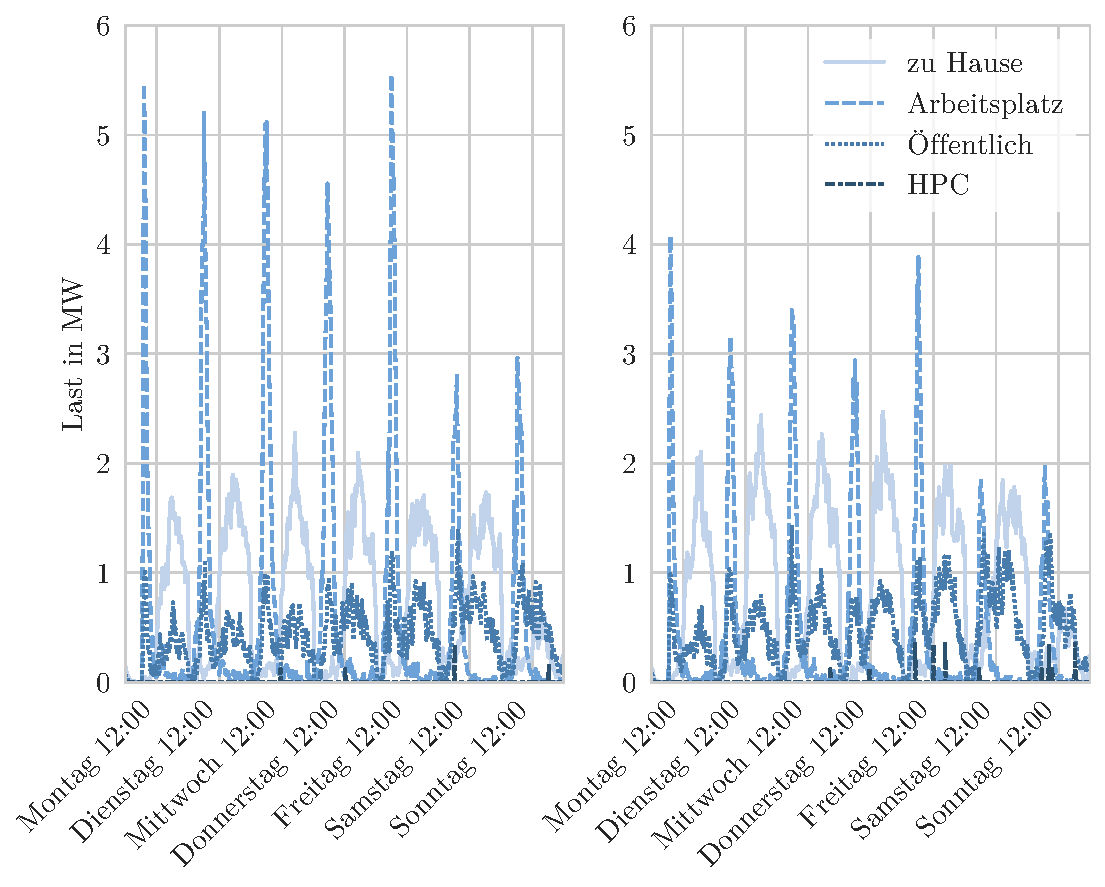
\includegraphics[width=\textwidth]{Bilder/example_load_profile}
    \caption[E-Pkw-Lastprofil für Referenz-Laden im Netz \num{176} über eine Woche im Antriebswende-Szenario und der \SzeFirmenparkplatz]{E-Pkw-Lastprofil (netzseitige Last; inkl. Umwandlungsverluste) für Referenz-Laden im Netz \(176_{\text{PV}}\) über eine Woche im Antriebswende-Szenario (links) und der \SzeFirmenparkplatz (rechts)}\label{fig:example_load_profile}
\end{figure} % TODO: Leistung statt Last

Die erstellten Fahrtprofile spiegeln ein plausibel erscheinendes Bild wider.
Die Lastgänge \zH und \Firmeparkplatz entsprechen den Ladevorgängen im privaten Bereich.
Unter dem Lastgang \oeffen sind hingegen alle öffentlichen Ladevorgänge mit Ausnahme der Schnellladevorgänge (\gls{HPC}) zusammengefasst.
Deutlich zu erkennen ist die hohe Gleichzeitigkeit am Vormittag sowohl am \Firmeparkplatz als auch im öffentlichen Raum, welche durch das Fahren zur Arbeit ausgelöst wird.
Auch die Rückkehr zum Wohnort ist ab dem frühen Nachmittag in den Lastgängen \zH und im öffentlichen Raum deutlich zu erkennen.
Die entsprechenden Dauerlastkurven für die Gemeinde über eine Woche (s. \autoref{fig:example_load_curve}) zeigen nochmals deutlich die dominante Rolle der Hochlastphase die Aufgrund der hohen Gleichzeitigkeit des Wegezwecks \Arbeit vor allem am \Firmeparkplatz aber auch im öffentlichen Raum auftritt.
Schnellladevorgänge treten unregelmäßig im Verlauf der Woche auf.
Vor allem am Sonntag kommt es zu deutlich geringeren Anteilen von Ladevorgängen \zH und am \Firmeparkplatzdot, wodurch das Flexibilisierungspotential am Wochenende geringer ausfällt.
Gegenüber dem Antriebswende-Szenario sinkt die Höchstlast in der \SzeFirmenparkplatzdot.
Jedoch sinkt auch das Flexibilisierungspotential bei gleichbleibendem Energiebedarf durch die Verschiebung der Ladevorgänge in den öffentlichen Raum.

\begin{figure}[H]
    \centering
    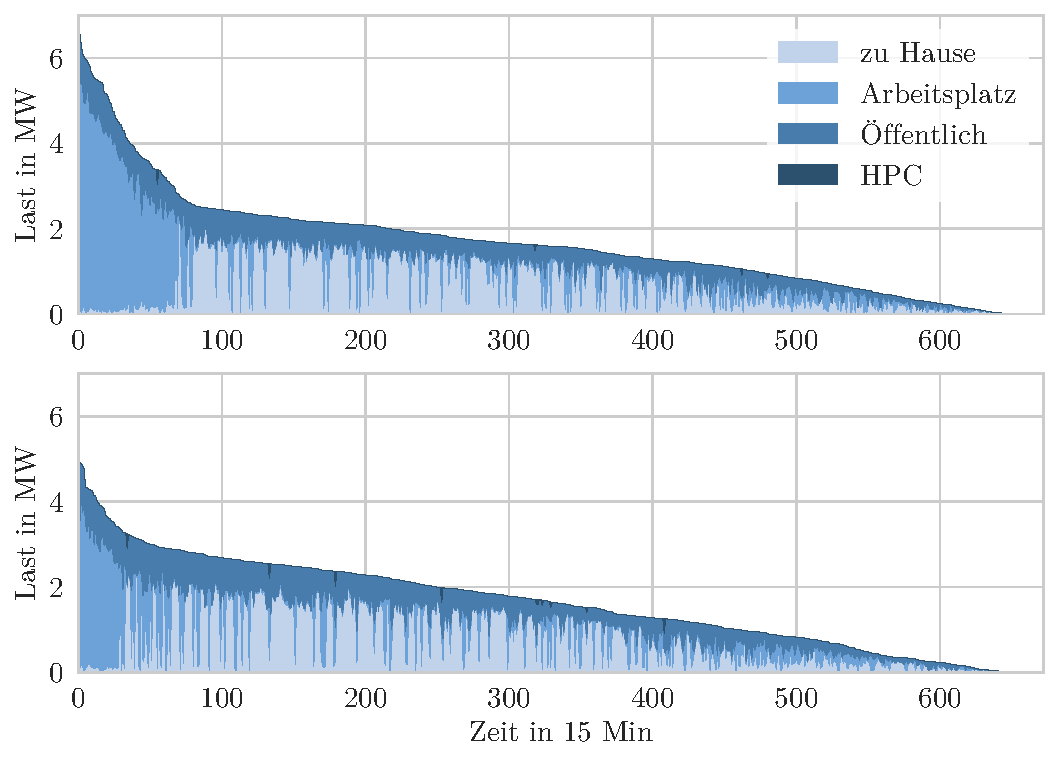
\includegraphics[width=0.9\textwidth]{Bilder/example_load_duration_curve}
    \caption{E-Pkw-Dauerlastkurve für Referenz-Laden im Netz \num{176} über eine Woche im Antriebswende-Szenario (oben) und der \SzeFirmenparkplatz (unten)}\label{fig:example_load_curve}
\end{figure} % TODO: Leistung statt Last

Zum Zeitpunkt der Erstellung der Fahrtprofile war es noch nicht möglich, einen längeren Zeitraum als eine Woche am Stück zu simulieren.
Durch die Zuordnung eines zufälligen Eingangs-\gls{SOC} für einige Fahrzeuge (s. \autoref{chap:simbev_theo}) fällt der Ladebedarf am Montag nicht deutlich aus der Reihe.
Jedoch kann hierdurch ein weiterer Effekt nitch verhindert werden.
Bei Fahrzeugen, welche weder einen festen Ladepunkt \zH oder am \Firmeparkplatz zugewiesen bekommen haben, fällt der \gls{SOC} im Laufe der Woche langsam ab.
Hierdurch kommt es durch die Abhängigkeit der Ladewahrscheinlichkeit vom \gls{SOC} zu einer Zunahme des Ladebedarfs im öffentlichen Raum über die Woche.
Es ist zu vermuten, dass dies weiterhin dazu führt, dass Ladevorgänge an Schnellladeinfrastruktur un­ter­re­prä­sen­tiert dargestellt werden.


\subsection{Verteilung der Ladevorgänge auf die Ladeinfrastruktur}\label{chap:distribute_demand_ev}

Die Verteilung der Ladevorgänge auf eine konkrete georeferenzierte Ladeinfrastruktur nach \autoref{chap:theo_distribution} liefert je Netzgebiet eine Vielzahl von unterschiedlichen Netzanschlusspunkten.
In \autoref{fig:cps_in_grid} finden sich beispielhaft die ermittelten Netzanschlusspunkte für Ladeinfrastruktur innerhalb des Netzgebietes \num{176} für das Antriebswende-Szenario für Ladeinfrastruktur zu Hause, am Arbeitsplatz und im öffentlichen Raum sowie für Schnellladeinfrastruktur (\gls{HPC}).
Es wird deutlich, dass die Ladeinfrastruktur zu Hause die meisten Netzanschlusspunkte aufweist, während für die Schnellladeinfrastruktur nur wenige Netzanschlusspunkte benötigt werden.
Weiterhin zeigt sich eine starke Konzentration der Ladeinfrastruktur in den bewohnten Regionen.

\begin{figure}[H]
    \centering
    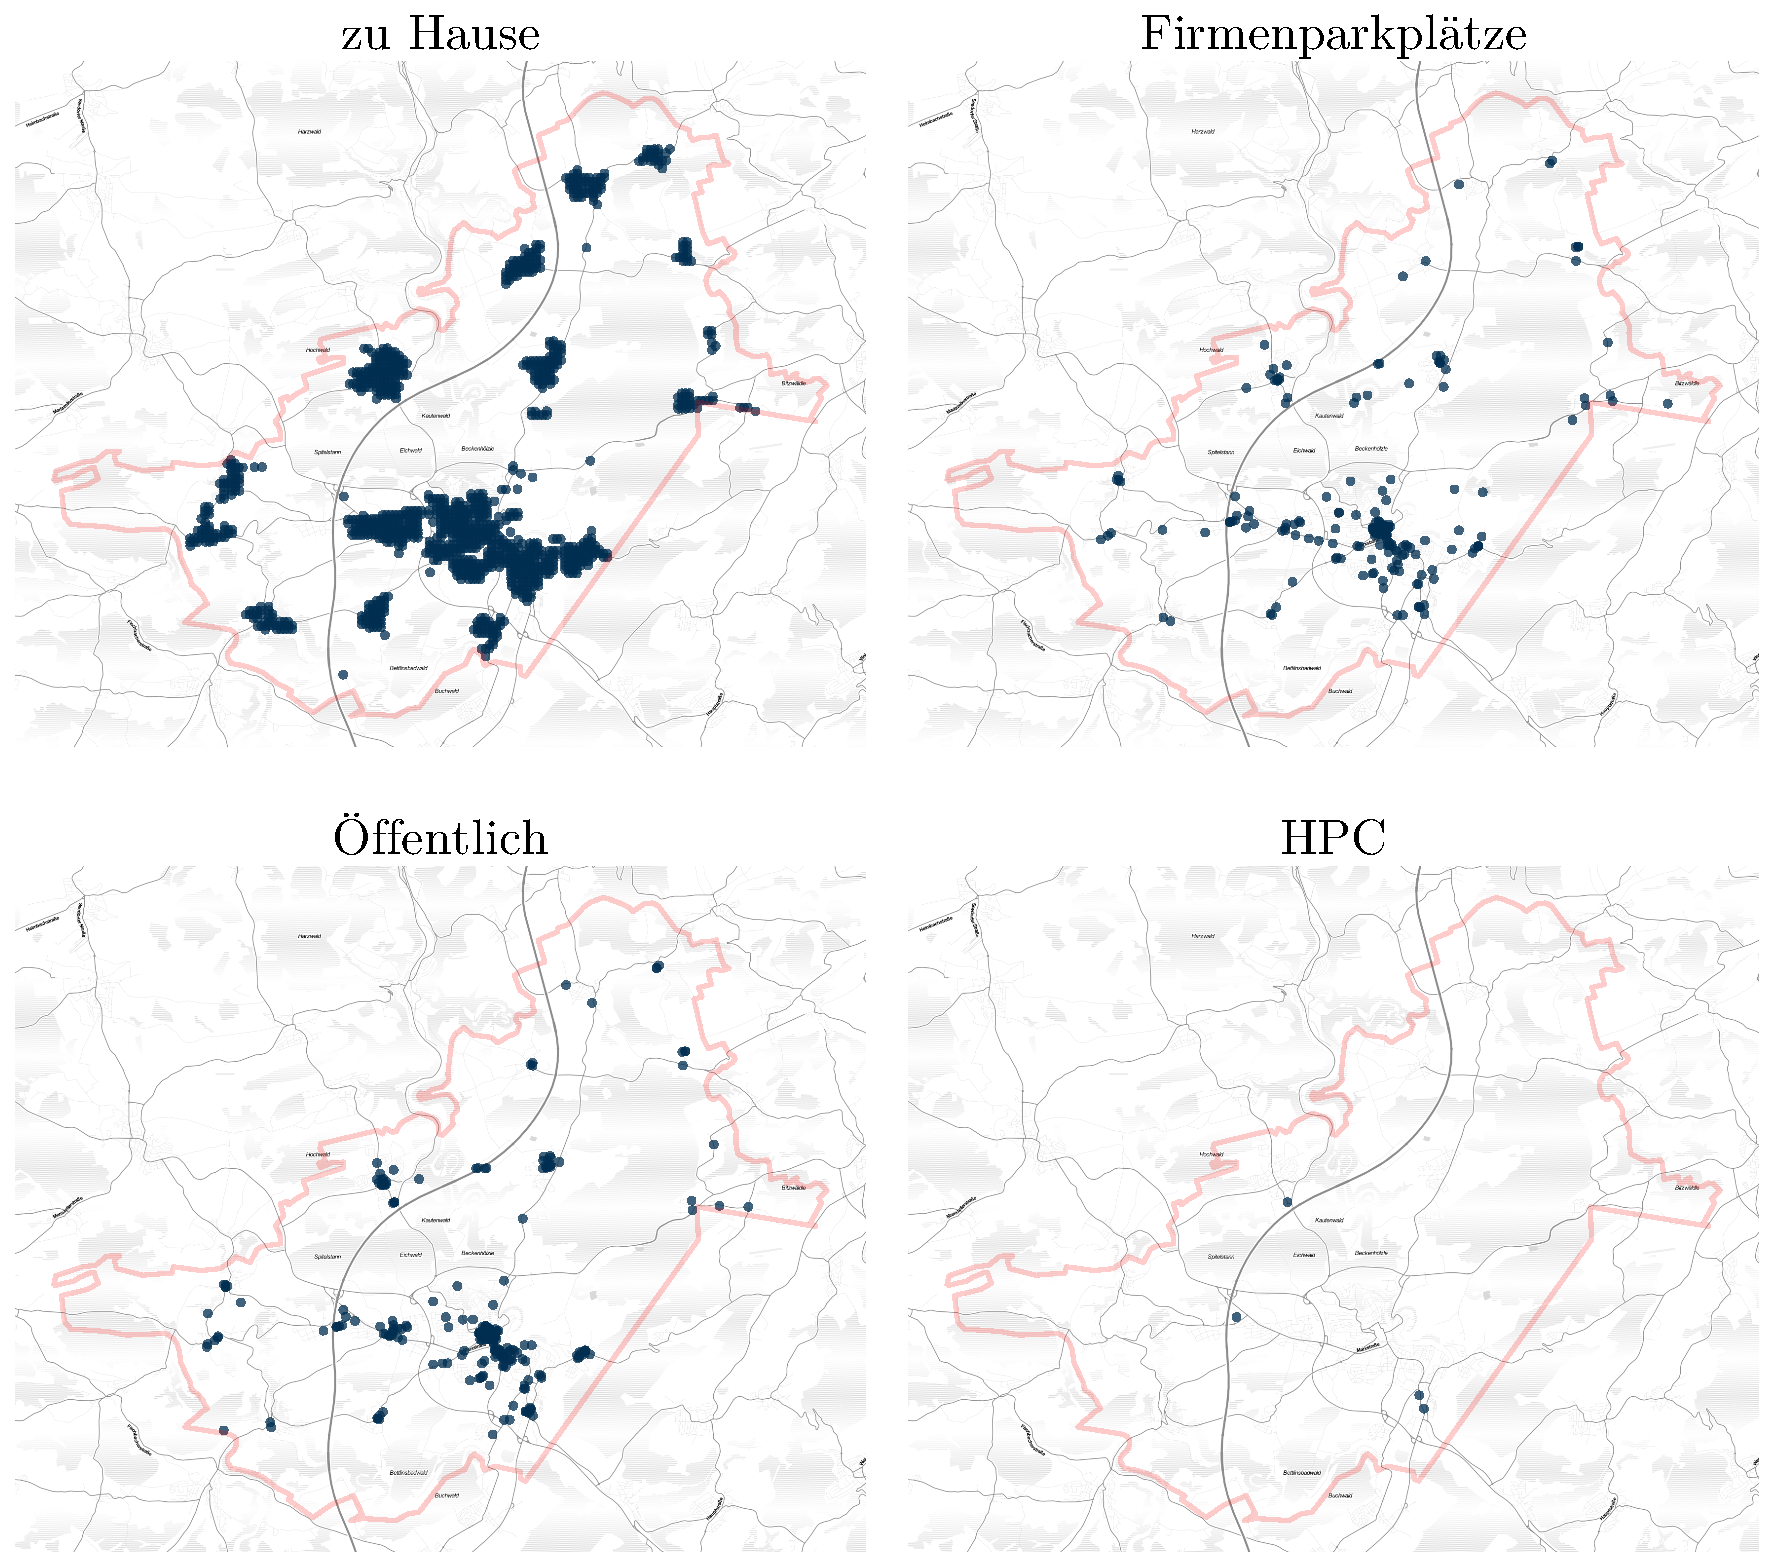
\includegraphics[width=\textwidth]{Bilder/cps_in_grid_176}
    \caption[Geographische Verteilung der ermittelten und zugewiesenen Netzanschlusspunkte für Ladeinfrastruktur im Netz \num{176} für das Antriebswende-Szenario je Lade use case]{Geographische Verteilung der ermittelten und zugewiesenen Netzanschlusspunkte für Ladeinfrastruktur im Netz \(176_{\text{PV}}\) für das Antriebswende-Szenario je Lade use case}\label{fig:cps_in_grid}
\end{figure}


\subsection{Ergebnisse der Implementierung der Ladestrategien}\label{chap:results_charging_strategies}

Im Rahmen der Netzuntersuchungen kommt den Zeitreihen der Last der \glspl{EPKW} die größte Bedeutung zu, da die Last und Erzeugung aller anderen Verbraucher und Erzeuger nicht veränderlich ist.
Das Ziel der Ladestrategien (s. \autoref{chap:theo_strategies}) ist es, die Netzbelastung möglichst gering zu halten.
Bei den Ladegruppen und reduzierten Laden soll dies durch ein präventives Lademanagement und bei dem Residuallast-Laden durch ein aktives Lademanagement erreicht werden.

\begin{figure}[H]
    \centering
    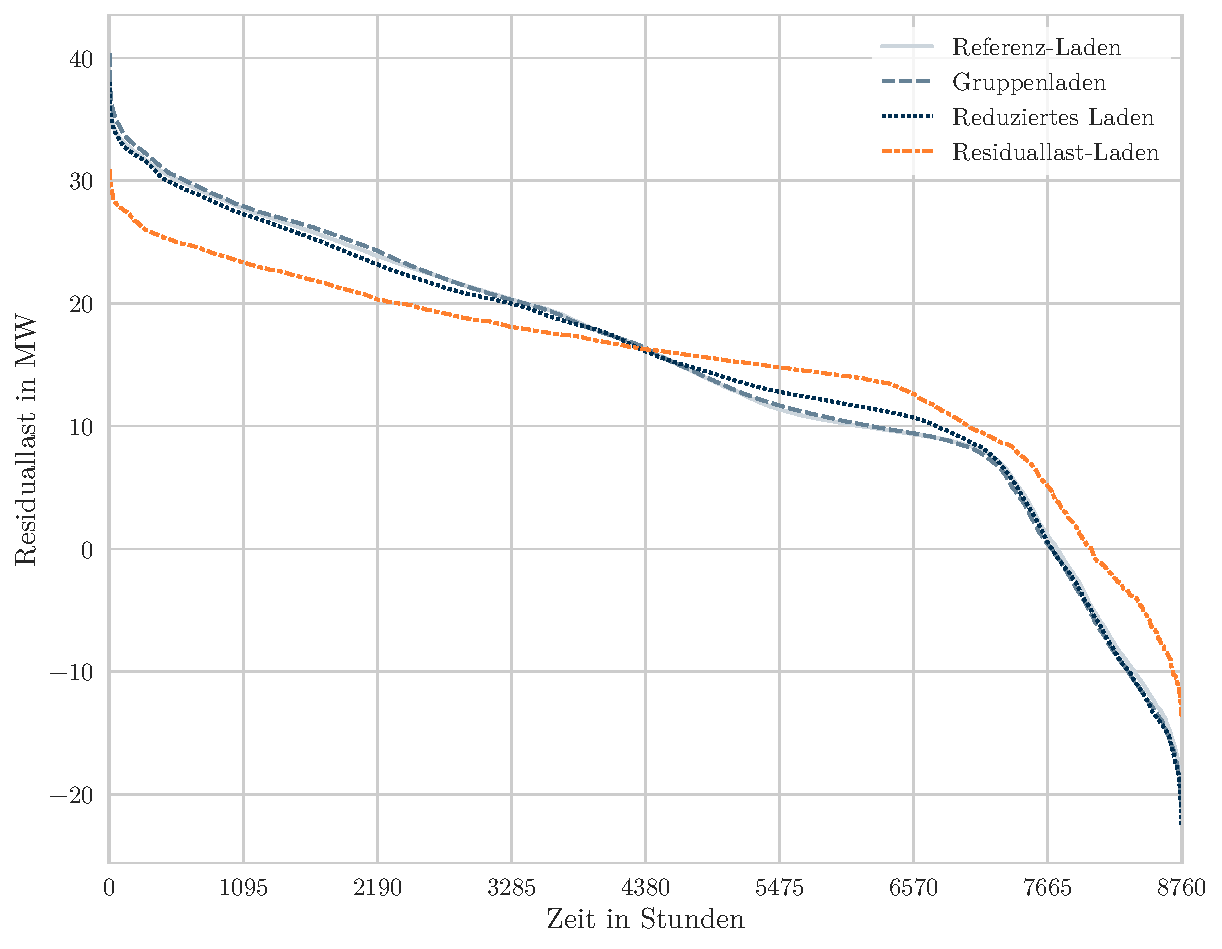
\includegraphics[width=1\textwidth]{Bilder/example_resiual_load}
    \caption{Residuallast im Netzgebiet \num{176} für das Antriebswende-Szenario}\label{fig:residual_load}
\end{figure}

\autoref{fig:residual_load} zeigt beispielhaft für das Netzgebiet \num{176} die Abhängigkeit der Residuallast von der Ladestrategie im Antriebswende-Szenario.
Dabei zeigt sich, dass vor allem die Residuallast-Ladestrategie zu einer klaren Glättung der Residuallastkurve führt, während sich bei den sonstigen Ladestrategien ein ähnliches Bild zeigt.
Dabei führen die Ladegruppen gegenüber dem Referenz-Laden sogar zu einem gegensätzlichen Effekt und zu einer Erhöhung der Spitzenlast im Last- und Rückspeisefall.
In \autoref{fig:residual_load_diff} ist die Veränderung der Residuallast über ein Jahr in Abhängigkeit von den verschiedenen Ladestrategien dargestellt.
Dabei zeigt die Darstellung der Referenz-Ladestrategie (oben links) die Residuallast über ein Jahr, während in den anderen drei Darstellungen die Differenz der jeweiligen Ladestrategie zum Referenz-Laden abgebildet wird.
Bei den Ladegruppen zeigt sich gegenüber dem Referenz-Laden eine deutlich stärkere Belastung am Vormittag und ein Abfallen der Belastung bis zum Mittag.
Am Nachmittag lässt sich in der Regel keine Differenz feststellen.
Bei der reduzierten Ladestrategie kommt es zu einer leicht reduzierten Residuallast im Verlauf des Tages, während die Residuallast Nachts leicht zunimmt.
Die stärksten Veränderungen werden bei der Residuallast-Ladestrategie festgestellt.
Da es sich bei dem Netzgebiet \num{176} um ein \gls{PV}-dominiertes Netz handelt, kommt es zu einer starken Verschiebung der Ladevorgänge in die Mittagszeit.
Auch kommt es zu einer deutlichen Verschiebung der Last in die Schwachlastzeit nach Mitternacht, während die Residuallast am Vor- und Nachmittag abnimmt.
Da auf diese weise jedoch nur Aussagen über das komplette \gls{MS}-Netzgebiet getroffen werden können, kann hier draus noch keine Aussage über die Belastung der einzelnen Betriebsmittel getroffen werden.

\begin{figure}[H]
    \centering
    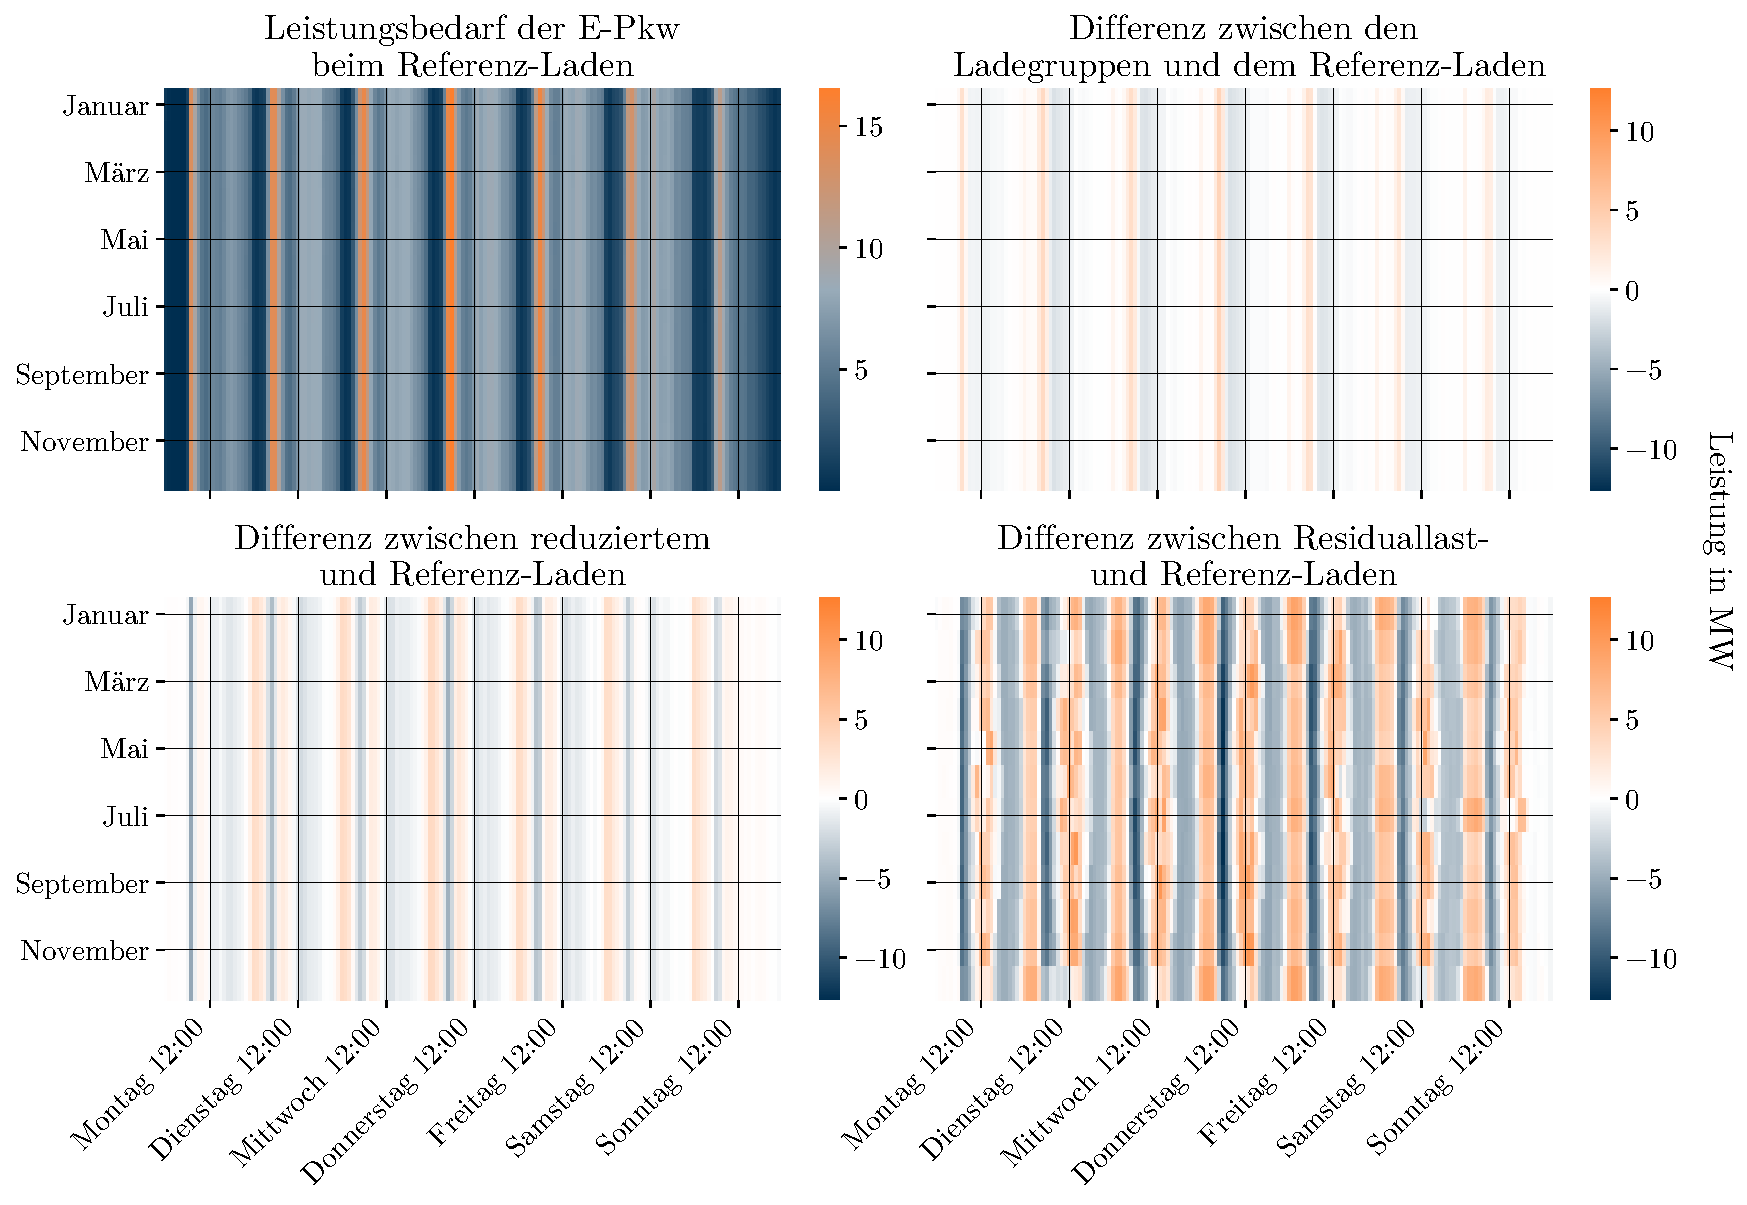
\includegraphics[width=\textwidth]{Bilder/residual_load_diff}
    \caption[Veränderung des durchschnittlichen stündlichen Leistungsbedarfs von E-Pkw je Wochentag im Netz \num{176} für das Antriebswende-Szenario über ein Jahr in Abhängigkeit von der Ladestrategie]{Veränderung des durchschnittlichen stündlichen Leistungsbedarfs von E-Pkw je Wochentag im Netz \(176_{\text{PV}}\) für das Antriebswende-Szenario über ein Jahr in Abhängigkeit von der Ladestrategie}\label{fig:residual_load_diff}
\end{figure}

% TODO: Eventuell Auswertung, wie sich die Residuallast durch das Residuallast-Laden verändert bei den unterschiedlichen Netzgebieten und Szenarien
% TODO: Bubble maps


\subsection{Abregelungsbedarf innerhalb der untersuchten Netzgebiete}

